\documentclass{beamer}\usetheme{boxes}

\usepackage{amsmath,hyperref,bbding,listings,url}
\usepackage{todonotes}

\newcommand{\bskip}{\\~\\}

\newcommand{\checkitem}{\item[\Checkmark]}
\newcommand{\xitem}{\item[\XSolidBrush]}
\newcommand{\mehitem}{\item[$\approx$]}
\newcommand{\easyframe}[2]{\frame{\frametitle{#1}
#2
}}

\lstdefinelanguage{scala}{morekeywords={class,object,trait,extends,with,new,if,while,for,def,val,var,this,override},
otherkeywords={->,=>},
%procnamekeys={def,.},
sensitive=true,
keywordstyle=\color{magenta},
commentstyle=\color{green},
identifierstyle=\color{blue},
%procnamestyle=\color{black},
morecomment=[l]{//},
morecomment=[s]{/*}{*/},
morestring=[b]"}
% Default settings for code listings
\lstset{frame=tb,language=scala,aboveskip=3mm,belowskip=3mm,
showstringspaces=false,columns=flexible,basicstyle={\small\ttfamily}}
% handle tilde characters
\lstset{literate=%
{~}{\url{~}}1
}


\author[CABP-BHS]{Carl~A.~B.~Pearson \&\ Burton~H.~Singer}
\institute[UF]{University of Florida, Emerging Pathogens Institute}
\usepackage{Sweave}
\begin{document}
\input{template-concordance}
\title{MURI 2013 Review, Part I}
\institute[University of Florida]{Emerging Pathogens Institute, University of Florida}

\frame{\titlepage}

\easyframe{Overview}{
\begin{itemize}
\item<1-> our focus: simulation approaches,
\item<2-> intra-MURI projects,
\item<3-> extra-MURI projects
\end{itemize}
% notes-notes-notes
}

\easyframe{Simulation Framework}{
Basic problem: lots of graph metrics, so what?
\begin{itemize}
  \item<2-> Limited closure of inductive-deductive loop
  \item<3-> Experimental options restricted
  \item<4-> So: want simple tool to simulate mechanics
\end{itemize}
% That is - does centrality matter?  Which centrality?  Does modularity matter?  What ties should be measured for that module?
% How do you tell? Conventional physical sciences experiments aren't available - I recently had an argument about the nature of the physical sciences vs social sciences.  We never agreed fully that there is a difference, but agreed that both follow the scientific method, and that the physical sciences have an easier time with measurement.  I think that latter point is pretty significant, she disagreed?  I'm not sure.
% Anyway - statistical outcomes aren't really the way the physical sciences like to do business.  But we can always do some more experiments, and the effects of history are quite short.  Less so with social phenomena.
}

\easyframe{Simulation Framework}{
``Simple'' == reduced syntax + piping connecting
\begin{itemize}
  \item<2-> initial graph generation
  \item<3-> dynamic graph evolution
  \item<4-> ``message'' passing and observation model
  \item<5-> agent-to-agent behavior
  \item<6-> agent-to-broadcast (and {\em vv}.) behavior
  \item<7-> interventions
  \item<8-> plus computational concerns (e.g., IO, cluster computation)
\end{itemize}
% notes-notes-notes
}

\easyframe{Simulation Framework Progress}{
\begin{itemize}
  \mehitem<2-> syntax
  \mehitem<3-> initial graph generation (on-going work w/ Ed/Edo re correlated interaction types)
  \xitem<4-> dynamic graph evolution
  \checkitem<5-> ``message'' passing and observation model
  \checkitem<6-> agent-to-agent behavior
  \xitem<7-> agent-to-broadcast (and vv.) behavior
  \xitem<8-> interventions
  \mehitem<9-> plus computational concerns (e.g., IO, cluster computation)
\end{itemize}
% notes-notes-notes
}

\begin{frame}[fragile]
\frametitle{Simulation Framework Syntax Progress}
\begin{lstlisting}
  def star
  [V <: Vertex[EdgeType,V]]
  (spokes : Seq[V], src: V) = {
    src <~> spokes
    src +: spokes
  }
\end{lstlisting}
so, e.g.
\begin{lstlisting}
  // A-E : Vertex
  val spoked = star(A, List(B, C, D, E))
  override def remix
  [V <: Vertex[EdgeType,V]]
  (vs : Seq[V], rate:Double) = {
    vs.dPairs.filter { _ => DoubleSrc.next < rate }.
    foreach { p => p._1 !~> p._2 }
  }
  remix(spoked,someRate) // directed edges flipped @ someRate 
\end{lstlisting}
% Scala offers nice mix of DSL (the graph operators),
% fully featured object-oriented + functional programming language
% unlike R (poor object support, stuck with expression mistakes from S)
% unlike C-family / Java, less boilerplate
\end{frame}

\easyframe{Results Reported at Sunbelt}{
Worked w/ Edo \&\ Ed to prepare basic simulated communications
\begin{itemize}
  \item simple graph generation:
  \begin{itemize}
    \item mixed interaction types
    \item households into communities
    \item clandestine manager + cliqued groups of subordinates
  \end{itemize}
  \item simple message passing - ``Good'' vs. ``Bad'', time-independent probabilities
\end{itemize}
% notes-notes-notes
}

\easyframe{Sample Population Graphs}{
\missingfigure{show mixed interaction types}
% notes-notes-notes
}

\easyframe{Sample Population Graphs}{
\missingfigure{highlight particular interaction types}
% notes-notes-notes
}

\easyframe{Sample Results Analysis}{
\missingfigure{toss in sunbelt example}
% notes-notes-notes
}

\easyframe{Aside on Results}{\begin{itemize}
\item<1-> Measured strategies as TPR and FPR over time, with fixed strategy criteria.

\item<2-> ROC could capture TPR vs FPR over criteria -- measure ROC scalar (e.g., discrimination) time evolution?

\item<3-> With several strategy knobs, even more complicated surface
\end{itemize}
% TPR = sensitivity, FRP = 1 - specificity
}

\easyframe{Intra-MURI Projects}{
\begin{itemize}
\item Airoldi / Kao -- implement more sophisticated conditional tie generators / activators
\item Lazer et al. -- simulate firm-induced vs background political donations
\item Shapiro -- identification with evolving SIMs, and using telephony data to parametrize graph generation
\end{itemize}
% notes-notes-notes
}

\easyframe{Intra-MURI Project: Lazer et al. Collaboration}{
Brief Detailed Note - Using Simulation Tool
\begin{itemize}
\item<2-> set up a population,
\item<3-> generate R and D stars,
\item<4-> sample a size distribution of firms, generate stars for each firm to individuals,
\item<5-> generate candidates / PACs with R or D affiliation,
\item<6-> star them to random subsets of firms,
\item<7-> each step\begin{itemize}
\item<7-> test for random donation (emit events from R/D stars)
\item<7-> have candidates / PACs solicit firms, which in turn organize events
\item<7-> employees respond to events with some probability, based on previous giving, personal affiliation vs event affiliation, etc
\end{itemize}
\end{itemize}
% We'll let Lazer's group speak to their specific work, and stick to what we're doing to support that.
}

\easyframe{Intra-MURI Project: Lazer et al. Collaboration}{
Analysis Idea
\begin{itemize}
\item intialize coordination belief network
\item Each step provides Bayesian update based on concordant / discordant giving
\item ROC discrimination calculated on percolation of coordination network
\end{itemize}
}

\easyframe{Extra-MURI Projects}{
\begin{itemize}
\item D. Bright, UNSW -- agent/process-based models of meth production
\item K. Carley, CMU -- adding broadcast/mean-field perspectives to agent-models
\item SAIC/L. Gerdes, USMA -- geo-temporal hashing, specifically estimating between-observation distribution
\item N. Roberts and S. Everton, NPGS -- dynamic growth of Noordin network
\item Assorted EPI -- cryptic infections (equivalent to rumor spreading source ID), using large Montreal WiFi access metadata
\end{itemize}
% notes-notes-notes
}

\usebackgroundtemplate{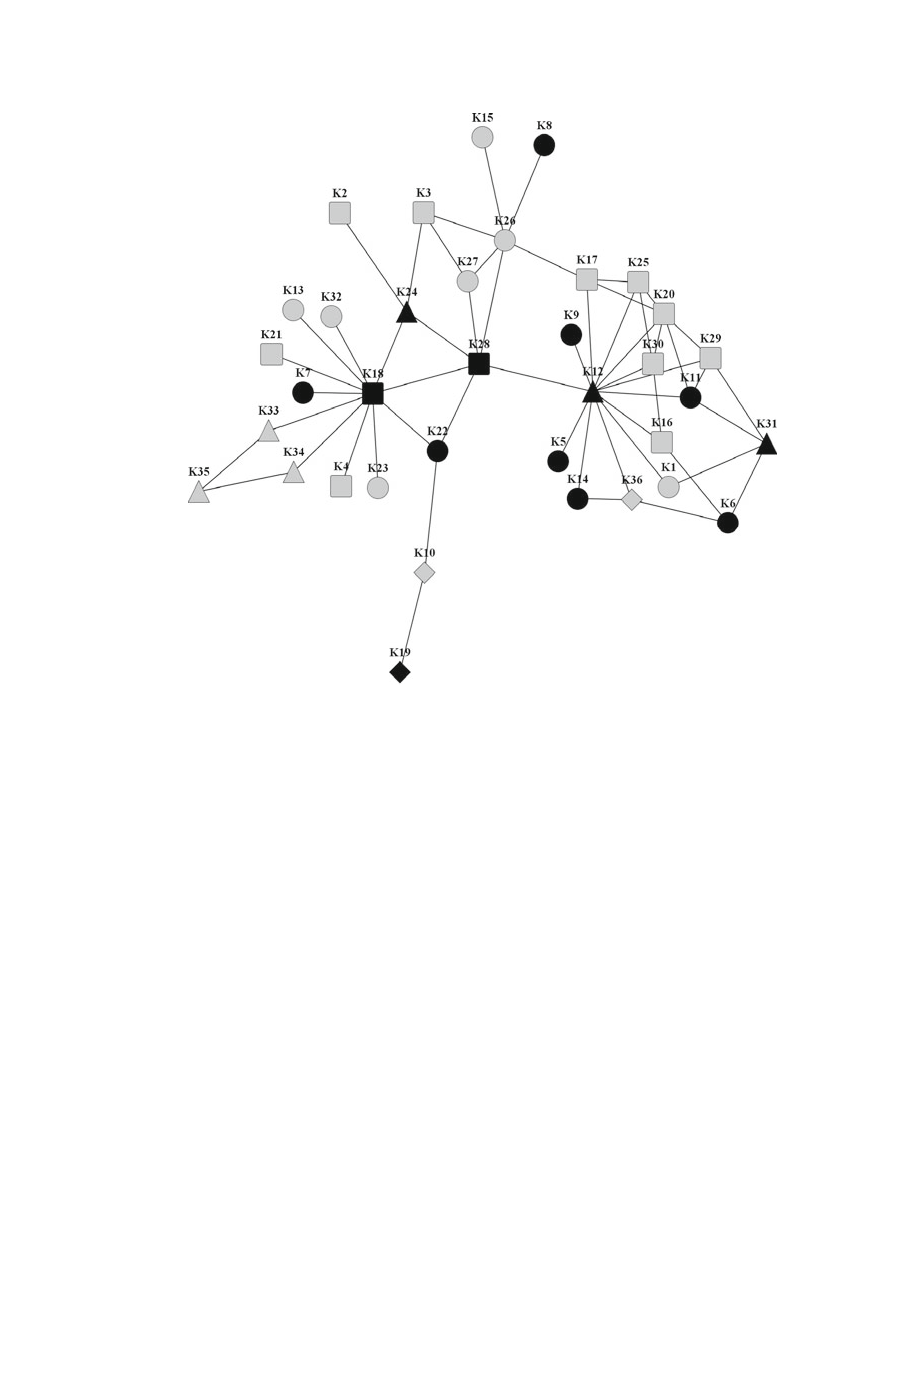
\includegraphics[width=0.9\paperheight,height=0.9\paperheight]{bright_roles.pdf}}
\easyframe{Extra-MURI Projects, David Bright}{
}
\usebackgroundtemplate{}

\easyframe{Extra-MURI Projects, Kathleen Carley}{
\begin{columns}[t]
\begin{column}{0.45\textwidth}
\begin{figure}
\begin{center}

\includegraphics[width=0.9\textwidth]{casos_logo_dark.png}
\end{center}
\end{figure}
\end{column}
\begin{column}{0.45\textwidth}
\begin{figure}
\begin{center}
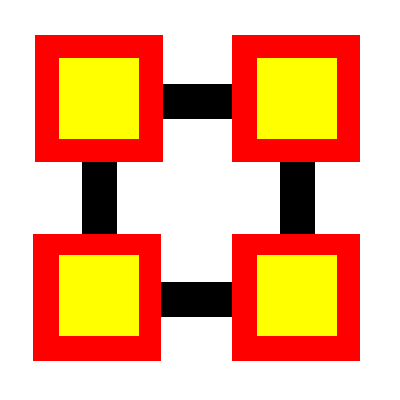
\includegraphics[width=0.9\textwidth]{ORA_logo.png}
\end{center}
\end{figure}
\end{column}
\end{columns}
% notes-notes-notes
}

\easyframe{Extra-MURI Projects, SAIC/Luke Gerdes}{
Work on geo-temporal hashing. 

They have good sifting tools to generate fuzzy co-location / time, but limited extrapolation.

Will be adding in some basic kinematics to expand that fuzz to unobserved periods, incorporate negative observations.
% notes-notes-notes
}

\easyframe{Extra-MURI Projects, Nancy Roberts \&\ Sean Everton}{
\missingfigure{Some of their Noordin results?}
% notes-notes-notes
}

\easyframe{Extra-MURI Projects, EPI}{
Mostly focused on large, anonymized data set of Montreal municipal WiFi access.

Tracking spread of cryptic pathogen analogous to tracking rumor to source
% notes-notes-notes
}

\end{document}
